\chapter{Algorithms}

The final chapter collects a few of the more important numerical algorithms and solvers used in the \mchem{} software, with some comments on the implementation details.

\section{Direct Inversion of The Iterative Subspace \label{sec:DIIS}}

The direct inversion of the iterative subspace (DIIS) method is an acceleration technique for solvers of nonlinear equations, originally introduced by Pulay \cite{Pul1980} in the context of the self-consistent field method. It has also found use in the solution of  the coupled cluster amplitude equations via Newton-Raphson methods, as well as in the Davidson diagonalization procedure. 

At a given iteration $i$, the DIIS method tries to find a set of coefficients $c_i$ such that the sum of the $m$ previous error vectors 
\begin{equation}
\mbf{e}_{i+1} = \sum_{i=0}^m c_i \mbf{e}_i
\end{equation}
\noindent approximates the null vector in a least-squares sense. The new coefficients are then used to extrapolate the solution $\mbf{p}$ for the next iteration using the current set of solution vectors:
\begin{equation}
\mbf{p}_{i+1} = \sum_{i=0}^m c_i \mbf{p}
\end{equation} 
\noindent In the classical DIIS scheme, the coefficients are furthermore required to sum to one 
\begin{equation}
\sum_i^m c_i = 1
\label{eq:DIIS_CONSTRAINT}
\end{equation}
\noindent Finding the coefficients thus corresponds to minimizing the Lagrangian subject to the constraint \ref{eq:DIIS_CONSTRAINT}:
\begin{equation}
\mathcal{L} = \mbf{c}\pdg \mbf{B} \mbf{c} - \lambda \left( 1 - \sum_i^m c_i \right)
\end{equation}
\noindent where $\mbf{B}$ is the matrix (or \emph{subspace})
containing the overlaps
\begin{equation}
B_{ij} = \sbraket{e_i}{e_j}
\end{equation}
\noindent Minimizing $\mathcal{L}$ with respect to $\mbf{c}$ gives
\begin{equation}
\frac{\partial \mathcal{L}}{\partial c_k} = 2 \sum_i^m c_i B_{ki} - \lambda = 0
\end{equation}
\noindent which then reduces to the matrix equation
\begin{equation}
\begin{pmatrix}
B_{00} & B_{01} & \ldots & B_{0m} & -1 \\
B_{10} & B_{11} & \ldots & B_{1m} & -1 \\
\vdots & \vdots & \ddots & \vdots & \vdots \\
B_{m0} & B_{m1} & \ldots & B_{mm} & -1 \\
-1 & -1 & \ldots & -1 & 0
\end{pmatrix}
\begin{pmatrix}
c_0 \\
c_2 \\
\vdots \\
c_m \\
\lambda 
\end{pmatrix}
=
\begin{pmatrix}
0 \\ 0 \\ \vdots \\ 0 \\ -1
\end{pmatrix}
\end{equation}
\noindent The system can be solved by inverting the subspace matrix (hence the name DIIS). 
The DIIS method is straight-forward to implement. Algorithm \ref{algo:DIIS} gives a summary for the method as it is used in the SCF procedure. 
The exact form of the error vector (or \emph{residual}) depends on the nature of the problem. In the general case, one can use the quantity
\begin{equation}
\mbf{e}_i = \mbf{e}_i - \mbf{e}_{i-1}
\end{equation}
\noindent In the case of the SCF method, the commutator relationship may be used instead:
\begin{equation}
\mbf{e}_i = \mbf{F}_i \mbf{P}_i \mbf{S} - \mbf{S} \mbf{P}_i \mbf{F}_i 
\end{equation}
In some cases, it is beneficial to remove some error vectors from the subspace to avoid linear dependencies. One can either remove the first error vector, or the vector with the largest norm. In most quantum chemistry software packages, the maximum DIIS space is set between 8 and 12. 

\begin{algorithm}
Compute the new Fock matrix $\mbf{F}_i$ for the current iteration $i$ using the density matrix $\mbf{P}_i$
\\
Compute the error vector $\mbf{e}_i = \mbf{F}_i \mbf{P}_i \mbf{S} - \mbf{S} \mbf{P}_i \mbf{F}_i$
\\
Add the error vector $\mbf{e}_i$ and the $\mbf{F}_i$ to the trial vectors. If the number of trial vectors is larger than a given threshold \textrm{DIIS\_MAX\_SUBSPACE}, remove  the first vector in the sets $\{\mbf{F}\}$ and $\{\mbf{e}\}$, or erase entry $k$ where $\mbf{e}_k$ is the error with the largest norm.
\\
Compute the overlap matrix $\mbf{B}$ and minimize the Lagrangian
\\
Compute a new Fock matrix using the new coefficients $\mbf{F}_{i+1} = \sum_i^m c_i \mbf{F}_i$, and diagonalize it to get the new density matrix $\mbf{P}_{i+1}$. 
\\
Increment $i$, begin new cycle
\caption{DIIS method for SCF}
\label{algo:DIIS}
\end{algorithm} 

\section{Davidson Diagonalization \label{sec:DAV}}

Eigenvalue problems involving large, symmetric matrices are ubiquitous in electronic structure theory. Due to the steep scaling in the number of elements, a full diagonalization is often not possible. Fortunately, in most cases the interest lies only in a few select eigenvalues, rather than the whole spectrum, and iterative methods may be used that avoid storing the whole matrix. Davidson's diagonalization procedure \cite{Dav1975} was originally introduced to extract the first few eigenvalues CI matrix, and is mainly used for eigenvalue problems of large, sparse, diagonally dominant matrices. Davidson's method is part of a larger category called \emph{Krylov subspace} methods. Krylov subspaces help to find approximate solutions to a higher-dimensional problem by projecting the matrix onto a smaller subspace that fits in memory. Other methods in this family include the Lanczos and Arnoldi algorithm, which also find uses in quantum chemistry \cite{Cor2012}.

\subsection{Davidson-Liu Method}

The Davidson method builds up an iterative subspace representation of the full matrix which corresponds to the overlap $\sbraket{r_i}{u_j}$ between the current set of trial vectors $\mbf{u}$ and the set of matrix-vector products $\mbf{r} = \mbf{A} \mbf{u}$. Diagonalizing this subspace matrix gives a set of approximate eigenvalues and eigenvectors. New trial vectors are constructed using the preconditioned residual. A \emph{preconditioner} helps to "steer" the problem into the right direction by better approximating the matrix $\mbf{A}$ and thus speeding up convergence. In the original paper, Davidson uses $\mbf{M} = \mbf{D} - \lambda \mbf{I}$ as the preconditioner, where $\mbf{D}$ is the exact diagonal of the matrix. If constructing the diagonal is too expensive, the \emph{Olsen preconditioner} may be used as an alternative, which approximates the diagonal to zeroth order \cite{Ols1990}. For example, the diagonal of the singles-singles block is then simply given by the MO energy differences $D_{ia} = \eps_i - \eps_a$. Other more sophisticated preconditioners have also been investigated \cite{Mor1990}. 

The quality of the starting guess vectors also influences convergence rate. In most quantum chemistry programs, they are constructed by considering the exact or approximate matrix diagonal $\mbf{D}$. The entries of $\mbf{D}$ are ordered from highest to lowest norm. The first guess vector is then generated by putting a 1 on the position of the matrix element with the highest norm, with the rest of the elements set to 0. The second, third, ... eigenvectors are constructed in a similar way. Eigenvectors from a lower order calculation can also be used as a starting guess for higher order methods (e.g. using CIS eigenvectors for ADC(2)). 

The Davidson method was originally a single-root method, i.e. each root needed a separate optimization. A \emph{blocked} version was proposed by Liu \cite{Liu1978}, which allows to optimize multiple roots at once. The blocked Davidson-Liu method as implemented in \mchem{} is given in Algorithm \ref{algo:DAVIDSON}. If only a single root is needed, the loops over the states are restricted to a single index instead, where $i_{root}$ corresponds to the desired root index. 

Furthermore, the Davidson procedure can be modified such that it follows eigenvectors that have a desired structure. The so-called \emph{root-homing} procedure \cite{But1976} reorders the eigenvalues and eigenvectors at each iteration according to overlap criteria. If one wishes to preserve the structure of the initial guesses, root-homing is essential. This modification to the Davidson algorithm is not implemented in \mchem{}.

While the Davidson algorithm avoids storing the whole matrix, it still needs to save the trial vectors and matrix-vector products. As the subspace grows, so does the number of vectors, which might become a memory bottleneck. To limit the number of vectors, the Davidson subspace can be collapsed and a new set of vectors can be formed according to
\begin{equation}
\mbf{u}'_i = \sum_j^{n_{dav}} V_{ji} \mbf{u}_j
\label{eq:COLLAPSE1} 
\end{equation}
\noindent where $\mbf{V}$ are the eigenvectors of the subspace matrix. This is followed by a normalization step
\begin{equation}
\mbf{u}^{new}_i = \frac{\mbf{u}'_i}{\vnorm{\mbf{u'}_i}}
\label{eq:COLLAPSE2}
\end{equation}
\noindent Subspace collapse allows to formulate a better estimate of the total memory requirements of the procedure. 

\begin{algorithm}
\setstretch{1.1}
\KwIn{Number of desired roots $n_{root}$, guess vectors $\mbf{U} = \{ \mbf{u}_i \}$, convergence threshold $d_{conv}$, (approximate) diagonal $\mbf{D}$, matrix-vector product function \textrm{mvp\_func()}}
\KwOut{Converged eigenvectors $\{\mbf{v}_i \}$ and eigenvalues $\{\omega_i \}$}

\While{not converged}{
Compute all the matrix-vector products which have not yet been computed
\begin{equation*}
\mbf{r}_{\oli} = \textrm{mvp\_func}(\mbf{u}_{\oli})
\end{equation*}
\\
Form the subspace matrix 
\begin{equation*}
A_{\oli\olj} = \mbf{r}_{\oli} \cdot \mbf{u}_{\olj} 
\end{equation*}
\\
Diagonalize $\mbf{A}$ to get the eigenvectors $\mbf{V} = \{\mbf{v}_{\oli} \}$ and eigenvalues $\{\omega_{\oli} \}$
\\
Compute the $n_{root}$ residuals 
\begin{equation*}
\boldsymbol{\rho}_i = \mbf{r}_{\olj} V_{\olj i}  - \mbf{u}_{\olj} V_{\olj i} \omega_{i}  
\end{equation*}
\\
Root $i$ has converged if $\vnorm{\boldsymbol{\rho}_i} < d_{conv}$ or $\left\lvert V(n_{dav}-1,i) \right\rvert < d_{conv}$ 
\\
If all roots have converged, then break, else continue.
\\
Compute the correction vectors $\{\mbf{e}_i\}$
\begin{equation*}
\mbf{e}_i = \frac{\boldsymbol{\rho}_i}{\mbf{D} - \omega_i \mbf{I}}
\end{equation*}
\\
Compute a new set of vectors $\{\mbf{b}_i\}$ by Gram-Schmidt orthogonalization of $\{\mbf{d}_i\}$ against the current set of $\{\mbf{u}_{\oli}\}$ 
\\
Normalize the new vectors $\{\mbf{b}_i\}$ and add all vectors to $\{\mbf{u}_{\oli}\}$ for which $\vnorm{\mbf{b}_i}/\vnorm{\mbf{d}_i}$ are above 1e-3 (to remove linear dependencies)
\\
If the size of the Davidson subspace $n_{dav}$ is above a given threshold, collapse the subspace and form a new set according to Equations \ref{eq:COLLAPSE1} and \ref{eq:COLLAPSE2}
} % end while

The final eigenvalues are equal to the eigenvalues of the last subspace matrix. The final eigenvectors $\{\mbf{v}_i\}$ are formed according to Equations \ref{eq:COLLAPSE1} and \ref{eq:COLLAPSE2} using the trial vectors $\{\mbf{u}_i\}$ and the eigenvectors of the subspace matrix 

\caption{Davidson-Liu Algorithm. Indices $i,j,k...$ implicitly loop over the number of roots $n_{roots}$, and indices $\oli, \olj, \olk, ...$ implicitly loop over the whole Davidson subspace $n_{dav}$.}
\label{algo:DAVIDSON}
\end{algorithm}

\subsection{Modified Davidson Method for the Pseudo-Eigenvalue Problem}

When using doubles-folding in the context of the ADC(2) or CC2 method (section \ref{sec:ADC_DAV}), the effective matrix $\mbf{A}_{eff}$ becomes dependent on its own eigenvalues:
\begin{equation}
\mbf{A}_{eff}(\omega) \mbf{v} = \omega \mbf{v}
\end{equation}
\noindent In this case, the standard Davidson method does not work, and needs to be modified to be able to solve this pseudo-eigenvalue problem. Different approaches have been proposed over the years, but are each based on similar principles \cite{Kat2009,Win2011}. The modified Davidson algorithm is given in Algorithm \ref{algo:PSEUDODAVIDSON}, as implemented in \mchem{}. 

The algorithm is split into \emph{macro} and \emph{micro} iterations, which are state-specific. The micro-iterations corresponds to the standard single-root Davidson iterations for diagonalizing an effective matrix $\mbf{A}_{eff}(\omega_i)$ with \emph{fixed} eigenvalue $\omega_i$. When the procedure has converged, $\omega_i$ is set to the new eigenvalue $\omega_i'$, and a new Davidson procedure, or macro-iteration commences with the effective matrix $\mbf{A}_{eff}(\omega_i)$. The macro-iterations are repeated until the eigenvectors have converged to a certain threshold. The individual roots are then further converged using DIIS.

\begin{algorithm}
\setstretch{1.1}
\KwIn{Number of desired roots $n_{root}$, guess vectors $\{ \mbf{u}_i \}$ and eigenvalues $\{ \omega^{(0)}_i \}$, convergence threshold $d_{conv}$, (approximate) diagonal $\mbf{D}$, matrix-vector product function \texttt{mvp\_func()}}
\KwOut{Converged eigenvectors $\{\mbf{v}_i \}$ and eigenvalues $\{\omega_i \}$}
Set $\omega^{macro}_i$ to $\omega^{(0)}_i$ and start macro-iterations for each individual state $i$
\\
\While{not converged}{
	Perform Davidson diagonalization on the effective matrix $\mbf{A}(\omega^{macro}_i)$. Convergence is reached when the difference between eigenvalues $\omega^{micro}_i$ from subsequent micro-iterations is smaller than the total change since the start of the procedure, i.e. at iteration $n$:
\begin{equation*}
\texttt{abs} \left( \omega^{macro}_i - \omega^{micro}_i \vert_{\textrm{iter} = 0} \right) > \texttt{abs} \left( \omega^{micro}_i \vert_{\textrm{iter}=n} - \omega^{micro}_i \vert_{\textrm{iter}=n-1} \right)  
\end{equation*}
\\
If the residual $\boldsymbol{\rho}_i$ is smaller than 1e-3, break, else continue
\\
Set $\omega^{macro}_i$ to $\omega^{micro}_i$, and $\mbf{u}_i$ to $\mbf{v}^{micro}_i$
} % end while
Set $\omega_i$ to $\omega^{macro}_i$, start DIIS
\\
\While{not converged}{
	Compute the matrix-vector product $\mbf{r}_i = \texttt{mvp\_prod}(\mbf{u}_i,\omega_i)$
	\\
	Compute the residual
	\begin{equation*}
	\boldsymbol{\rho}_i = \frac{\mbf{r}_i - \omega_i \mbf{u}_i}{\vnorm{\mbf{u}_i}}
	\end{equation*}	 
	\\
	Compute the new eigenvalue $\omega_i$
	\begin{equation*}
	\omega_i = \frac{\mbf{u}_i \cdot \mbf{r}_i}{\vnorm{\mbf{u}_i}}
	\end{equation*}
	\\
	If $\vnorm{\boldsymbol{\rho}_i} < d_{conv}$, root $i$ has converged, break
	\\
	Compute the corrected vector $\mbf{b}_i$ according to
	\begin{equation*}	 
	\mbf{b}_i = \mbf{u}_i + \frac{\boldsymbol{\rho}_i}{\mbf{D}}
	\end{equation*} 
	\\
	Add $\boldsymbol{\rho}_i$ to the DIIS error vector space, and perform extrapolation on $\boldsymbol{b}_i$ to get a new guess vector $\mbf{u}_i$ 
} % end while

\caption{Modified Davidson algorithm with DIIS acceleration for pseudo-eigenvalue problems.}
\label{algo:PSEUDODAVIDSON}
\end{algorithm}

%\section{Boys Localization \label{sec:LOCORB}}

\section{Incomplete Cholesky Decomposition \label{sec:CHOLDEC}}

The Cholesky factorization decomposes a symmetric, positive definite (PD) matrix into a lower and upper triangular matrix:
\begin{equation}
\mbf{A} = \mbf{L} \mbf{L}^T
\label{eq:NONPIVCHOL}
\end{equation}
\noindent where $\mbf{L}$ has the same dimension as $\mbf{A}$. However, the Cholesky factorization, as defined in \ref{eq:NONPIVCHOL}, does not exist for positive semi-definite (PSD) matrices. To see the reason why, consider Algorithm \ref{algo:CHOL} for the standard Cholesky factorization. The loop runs over all columns $i$ of $\mbf{A}$  and involves divisions by the diagonal elements $L_{ii}$. For PSD matrices, some of these elements will be zero due to linear dependencies of the column vectors, and the operation is therefore not defined.

\begin{algorithm}
\setstretch{1.1}
\KwIn{Symmetric matrix $\mbf{A}$ with dimension $N$ by $N$}
\KwOut{Cholesky factors $\mbf{L}$}
$L_{00} \leftarrow \sqrt{A_{00}}$
\\
$L_{j0} \leftarrow \frac{a_{j0}}{L_{00}} \quad j \in [1:N]$
\\
$L_{ii} \leftarrow \sqrt{ A_{ii} - \sum_{k=0}^{i} L_{ik}^2} \quad i \in [1:N]$ 
\\
$L_{ji} \leftarrow \left( A_{ji} - \sum_{k=0}^{i} L_{ik} L_{jk} \right) / L_{ii} \quad i \in [1:N] \quad j \in [i+1:N]$
\caption{Cholesky decomposition without pivoting.}
\label{algo:CHOL}
\end{algorithm}
 
A PSD matrix is also called \emph{rank-deficient}. The rank of a symmetric matrix is equal to the number of linearly independent column vectors. The occupied atomic density matrix $\mbf{P}$ is an example of a rank-deficient matrix. The atomic orbital basis, with $N_{bas}$ functions, is often redundant and has linear dependencies, which translates to a lower rank $r < N_{bas}$ of the occupied density matrix. The rank of $\mbf{P}$ is equal to the number of occupied molecular orbitals. The atomic orbital overlap matrix $\mbf{S}$ is an example of a "numerically" positive semi-definite matrix. While the column vectors are not strictly linearly dependent from a mathematical point of view, they are linearly dependent in the sense of floating-point precision. The diagonals $L_{ii}$ are close to zero ($<$ 1e-5), which will lead to large values and reduced accuracy when dividing.  

The Cholesky factorization can be generalized to PSD matrices by introducing permutation matrices which pivot the columns and rows of $\mbf{A}$:
\begin{equation}
\mbf{P} \mbf{A} \mbf{P}^T = \mbf{L} \mbf{L}^T 
\end{equation}
\noindent or
\begin{equation}
\mbf{A} = \mbf{P}^T \mbf{L} \mbf{L}^T \mbf{P}
\end{equation}
\noindent where $\mbf{L}$ is a $N$ by $k$ lower triangular matrix with $k = rank(\mbf{A})$. The 
permutation matrices swap the diagonal entries $L_{ii}$, also known as \emph{pivots}, in a way that division by zero is avoided during the procedure. If the pivot is below a certain threshold, the procedure halts and the number of total iterations is equal to the rank of $\mbf{A}$. The \emph{incomplete} pivoted Cholesky factorization is therefore \emph{rank-revealing}. Other examples of rank-revealing decompositions include the pivoted QR decomposition, and the singular value decomposition.

The Cholesky decomposition with full pivoting is given in Algorithm \ref{algo:CHOLPIV}. It can also be used in cases where the matrix is nearly positive semi-definite ($N \approx rank(A)$) for extra numerical stability, e.g. the AO overlap matrix. In \mchem{}, the pivoted Cholesky factorization is used to obtain a set of localized Cholesky MO coefficients which help to reduce the prefactor of atomic orbital methods. 

\begin{algorithm}
\setstretch{1.1}
\KwIn{Symmetric matrix $\mbf{A}$ with dimension $N$ by $N$, threshold $d_{lindep}$}
\KwOut{Cholesky factors $\mbf{L}$ and the rank $r$ of $\mbf{A}$}
Initialize index vector $perm = \{0,1,2,...,N\}$
\\
\For{$i = 0$ \textbf{to} $N$}{
	Find maximum diagonal element $A_{max} = A_{jj}$
	\\
	Swap rows $i$ and $j$ of $\mbf{A}$
	\\
	Swap columns $i$ and $j$ of $\mbf{A}$
	\\
	Swap $perm(i)$ and $perm(j)$
	\\
	\uIf{$A_{max} < 0$}{
		Negative pivot element, the Cholesky decomposition is not possible
	} 
	\uIf{$abs(A_{max}) < d_{lindep}$}{
		$r = i+1$, break
	}
	$L_{ii} = \sqrt{A_{max}}$
	\\
	$L_{ki} =  A_{ki}/\sqrt{A_{max}} \quad k \in [i+1:N]$
	\\
	$A_{kl} = A_{kl} - L_{ki} L_{kl} \quad k,l \in [i+1:N]$
} % endfor 
Impose original order of the rows, set row $perm(i)$ of the new Cholesky matrix $\mbf{L}'$ to row $i$ of $\mbf{L} \quad i \in [0:r]$
\\
Set $\mbf{L}$ to $\mbf{L}'$

\caption{Incomplete Cholesky decomposition with full pivoting.}
\label{algo:CHOLPIV}
\end{algorithm}

\subsubsection{Comments}

It should be noted that pivoting destroys the banded structure of the matrix $\mbf{L}$ (Figure \ref{fig:LOCORB_CHOL}). In other words, the pivoted Cholesky factorization of a diagonally dominant, sparse matrix may not give sparse matrices $\mbf{L}$ in the block-diagonal form. Blocking significant elements together reduces the number of non-zero blocks, which is crucial for the performance of atomic orbital based methods. It is therefore necessary to reorder the columns of $\mbf{P^TL}$ at the end of the procedure. In \mchem{}, this is done by sorting the columns by their weight $n = (p_f - p_i) / 2$, where $p_i$ is the first significant element in the column, and $p_f$ is the last significant element. The block-diagonal form can then restored for $\mbf{L}$. 

The pivoted Cholesky decomposition in \mchem{} does not exploit sparsity and scales with $\mathcal{O}(N^2rank(A))$. While a sparse implementation could be considered, row and column pivoting often destroys sparsity patterns (also known as \emph{fill-in}) and leads to a lot of reordering within the sparse data structures. Pivoting needs to be applied in such a way that fill-in is reduced to keep scaling low. 

Finally, pivoting also negatively impacts parallelization when using MPI. When columns are swapped, this incurs additional communication overhead between processes. Moreover, global communication is necessary to communicate the position and value of the maximum diagonal element to each process, which further slows down the procedure. Efficient parallelization of matrix decompositions with pivoting is subject of current research \cite{Xia2016,Xia2017}.

\section{Laplace Transformation \label{sec:LAPLACE}}

The Laplace transformation is  a crucial step for formulating an orbital invariant MP2 energy expression, where the orbital energy denominator is converted to an exponential form 
\begin{equation}
\frac{1}{\eps_a + \eps_b - \eps_i - \eps_j } = \frac{1}{x} = \int_0^{\infty} e^{-xt} dt
\end{equation} 
\noindent The integral is then approximated by the Laplace quadrature
\begin{equation}
\frac{1}{x} = \sum_{\alpha = 0}^{k} \omega\pa e^{-xt\pa}  
\end{equation}
\noindent where $k$ is the number of quadrature points, $\omega\pa$ are the Laplace weights and $t\pa$ are the Laplace exponents. In their original paper, Häser and Almlöf \cite{Has1992} computed the Laplace parameters by least-squares minimization of the error distribution function
\begin{equation}
\eta_k (x,\omega\pa,t\pa) = \sum_{\alpha = 0}^k \omega\pa e^{-xt\pa} - \frac{1}{x}
\end{equation}
\noindent in the interval $[x_{min},x_{max}]$. Later, it was shown that the quadrature parameters can be computed at a much lower cost using a minimax approximation (MA) \cite{Tak2008}, which \emph{minimizes} the \emph{maximum} Chebychev norm
\begin{equation}
\delta_{k[1,R]}(\bar{\omega}\pa,\bar{t}\pa) = \max_{x \in [1,R]} \left\lvert \eta_k (x,\bar{\omega}\pa,\bar{t}\pa ) \right\rvert 
\end{equation}
\noindent with the scaled Laplace parameters $\bar{\omega} = \omega x_{min}$, $\bar{t} = t x_{min}$  in the new interval $[1,R]$ where $R = x_{max}/x_{min}$. The scaled Laplace coefficients in the minimax approximation are obtained by repeating the following two steps until self-consistency is reached:
\begin{enumerate}
\item Determine the $2k-1$ extremum points $x_i$ of the error distribution function \\ 
$\eta_k (x,\bar{\omega}\pa,\bar{t}\pa)$ with the current set of $\{\bar{\omega}\}$ and $\{\bar{t}\pa\}$
\item Optimize the $2k+1$ parameters $\{\bar{\omega}\pa\}$ and $\{\bar{t}\pa\}$ by solving the $2k+1$ non-linear equations
\begin{equation}
\eta_k (x_i,\bar{\omega}\pa,\bar{t}\pa) = (-1)^i \delta_{k[1,R]}(\bar{\omega}\pa,\bar{t}\pa)
\end{equation} 
\end{enumerate}
\noindent This procedure is also known as the Remez algorithm (RA). Each of the two steps are non-trivial to compute. The set of non-linear equations in step 2 can be solved by performing a Newton-Raphson minimization using pre-tabulated values of $\{\bar{\omega}\pa\}$ and $\{\bar{t}\pa\}$ as guesses for the first RA iteration. Step 1 is a bit more complicated, and is either solved (a) by first finding the nodal points $x_0$ of the error distribution function to compute the extremum points using Newton-Raphson \cite{Tak2008}, or (b) by finding the extremum points directly using the Newton-Maehly algorithm \cite{Hel2016}. For further details, the reader is referred to the original publications.

All calculations in this report use the robust minimax approximation as proposed by Helmich-Paris and Visscher \cite{Hel2016}. They have published their source code on GitHub (GitHub.com/bhelmichparis/laplace-minimax), which was in turn incorporated into the \mchem{} software.

\section{Cuthill-McKee}

The Cuthill-McKee (CM) algorithm finds a permutation $P$ of a sparse, symmetric matrix that minimizes its \emph{bandwidth} \cite{Cut1969}. A banded matrix is a matrix that has all significant elements clustered around the main diagonal. The bandwidth $k$ is defined as the smallest positive index for which
\begin{equation}
\min_k \left\lvert A(k,k) \right\rvert = 0 \qquad k \in [0,N]
\end{equation}
\noindent The CM algorithm reduces the bandwidth of a matrix by reordering the nodes of the corresponding adjacency or connectivity matrix $\mbf{C}$ (Algorithm \ref{algo:CM}). For a $N$-by-$N$ matrix, there are $N$ nodes. Node $i$ and $j$ are connected if the entry $(i,j)$ of the connectivity matrix is 1, and not connected if the entry is 0. Here, the \emph{degree} of a node is defined by the total number of connections, i.e. the row or column sum
\begin{equation}
degree(i) = \sum_j^N C(i,j)
\end{equation}
In the context of quantum chemistry, the nodes correspond to atoms in a molecule, and the connections to bonds. Reordering the indexing of the atoms based on the connectivity matrix of a molecule allows to significantly reduce the number of blocks needed to store quantities like the overlap matrix, density matrix or 2-electron repulsion integrals when using block-sparse matrix algebra by grouping close atoms together. Figure \ref{fig:RCM} shows how the connectivity matrix is reordered for the FW144 system using the reverse CM algorithm. Two atoms are "connected", if their are within 5 $a_0$ of each other.

\begin{figure}
\centering
\begin{minipage}{0.45\textwidth}
\centering
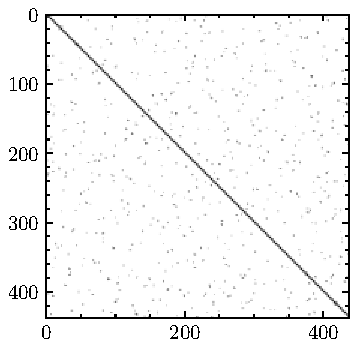
\includegraphics[width=\textwidth]{Pics/FW144_UNORDERED}
\end{minipage}
\begin{minipage}{0.45\textwidth}
\centering
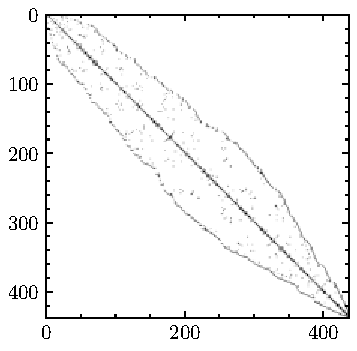
\includegraphics[width=\textwidth]{Pics/FW144_ORDERED}
\end{minipage}
\caption[Illustration of the Cuthill-McKee algorithm]{Connectivity matrix of FW144 before reordering (left), and connectivity matrix after applying the reverse Cuthill-McKee algorithm (right). Reducing the bandwidth allows to compress matrices and tensors in the AO basis into a much smaller space when using the block-sparse format.}
\label{fig:RCM}
\end{figure}

\begin{algorithm}
\setstretch{1.1}
\KwIn{Sparse symmetric matrix $\mbf{A}$ with dimension $N$ by $N$}
\KwOut{Reordered matrix $\mbf{A}$ with minimized bandwidth.}

Form the binary connectivity matrix $\mbf{C}$ of the input matrix
\\
Instantiate empty queue $Q$ and result array $R$
\\
\While{true} {
	Find node $p$ with minimum degree that is not yet in $R$, and put it into $R$
	\\
	Add all nodes to the queue that are connected to $p$
	\\
	\While{length of $Q \neq 0$}{
		Get fist node $q$ in queue, and pop it from queue
		\\
		\uIf{$q$ in $R$}{
		 	skip to next loop
		}
		\Else{
			add $q$ to $R$
		}
		Append all nodes connected to $q$ not yet in $R$ both to $R$ and $Q$
	} % end while q
	\uIf{size of $R = N$}{
		break
	}
} % end while R
Reorder the rows and columns of $\mbf{A}$ according to $R$ (standard Cuthill-McKee) or the reverse order of $R$ (reverse Cuthill-McKee)

\caption{(Reverse) Cuthill-McKee algorithm.}
\label{algo:CM}
\end{algorithm}

%\section{Quasi-Robust Density Fitting}

